
\chapter{Experimentálne vyhodnotenie}

V~tejto kaptiole predvedieme niekoľko vizualizácií, ako reálnych rRNA
sekundárnych štruktúr, tak aj menších, umelo vytvorených štruktúr
a na konci kapitoly zhrnieme hlavné nedostatky, ktoré naša aplikácia má.



\section{Experimenty na testovacích štruktúrach}

Už v predchádzajúcich kapitolách sme sa stretli s niekoľkými príkladmi vygenerovaných
štruktúr (vkladanie do hairpinu, stemu, alebo multibranch loop, ktoré sú
na obrázkoch \ref{obr:insert_circle_hairpin}, \ref{obr:insert_stem} a~\ref{obr:insert_multibranch}).

V~tejto časti sa budeme venovať umelo vytvoreným štruktúram, na ktorých ukážeme,
ako si náš program poradil s~dvoma po sebe idúcimi inverznými
operáciami - delete a~insert, po ktorých by sme chceli získať
naspäť pôvodnú vizualizáciu.

\begin{figure}[H]
  \centering
  \begin{subfigure}{0.3\textwidth}
%trim=left bottom right top
    \includegraphics[clip, trim=1cm 21cm 14cm 2.5cm, width=0.85\textwidth]{../img/alg/insert/2/multibranch-beg}
    \caption{}
    \label{obr:delete_insert_multibranch_stem_a}
  \end{subfigure}
  \begin{subfigure}{0.3\textwidth}
%trim=left bottom right top
    \includegraphics[clip, trim=0 21cm 15cm 2.5cm, width=0.85\textwidth]{../img/alg/insert/2/multibranch-del}
    \caption{}
    \label{obr:delete_insert_multibranch_stem_b}
  \end{subfigure}
  \begin{subfigure}{0.3\textwidth}
%trim=left bottom right top
    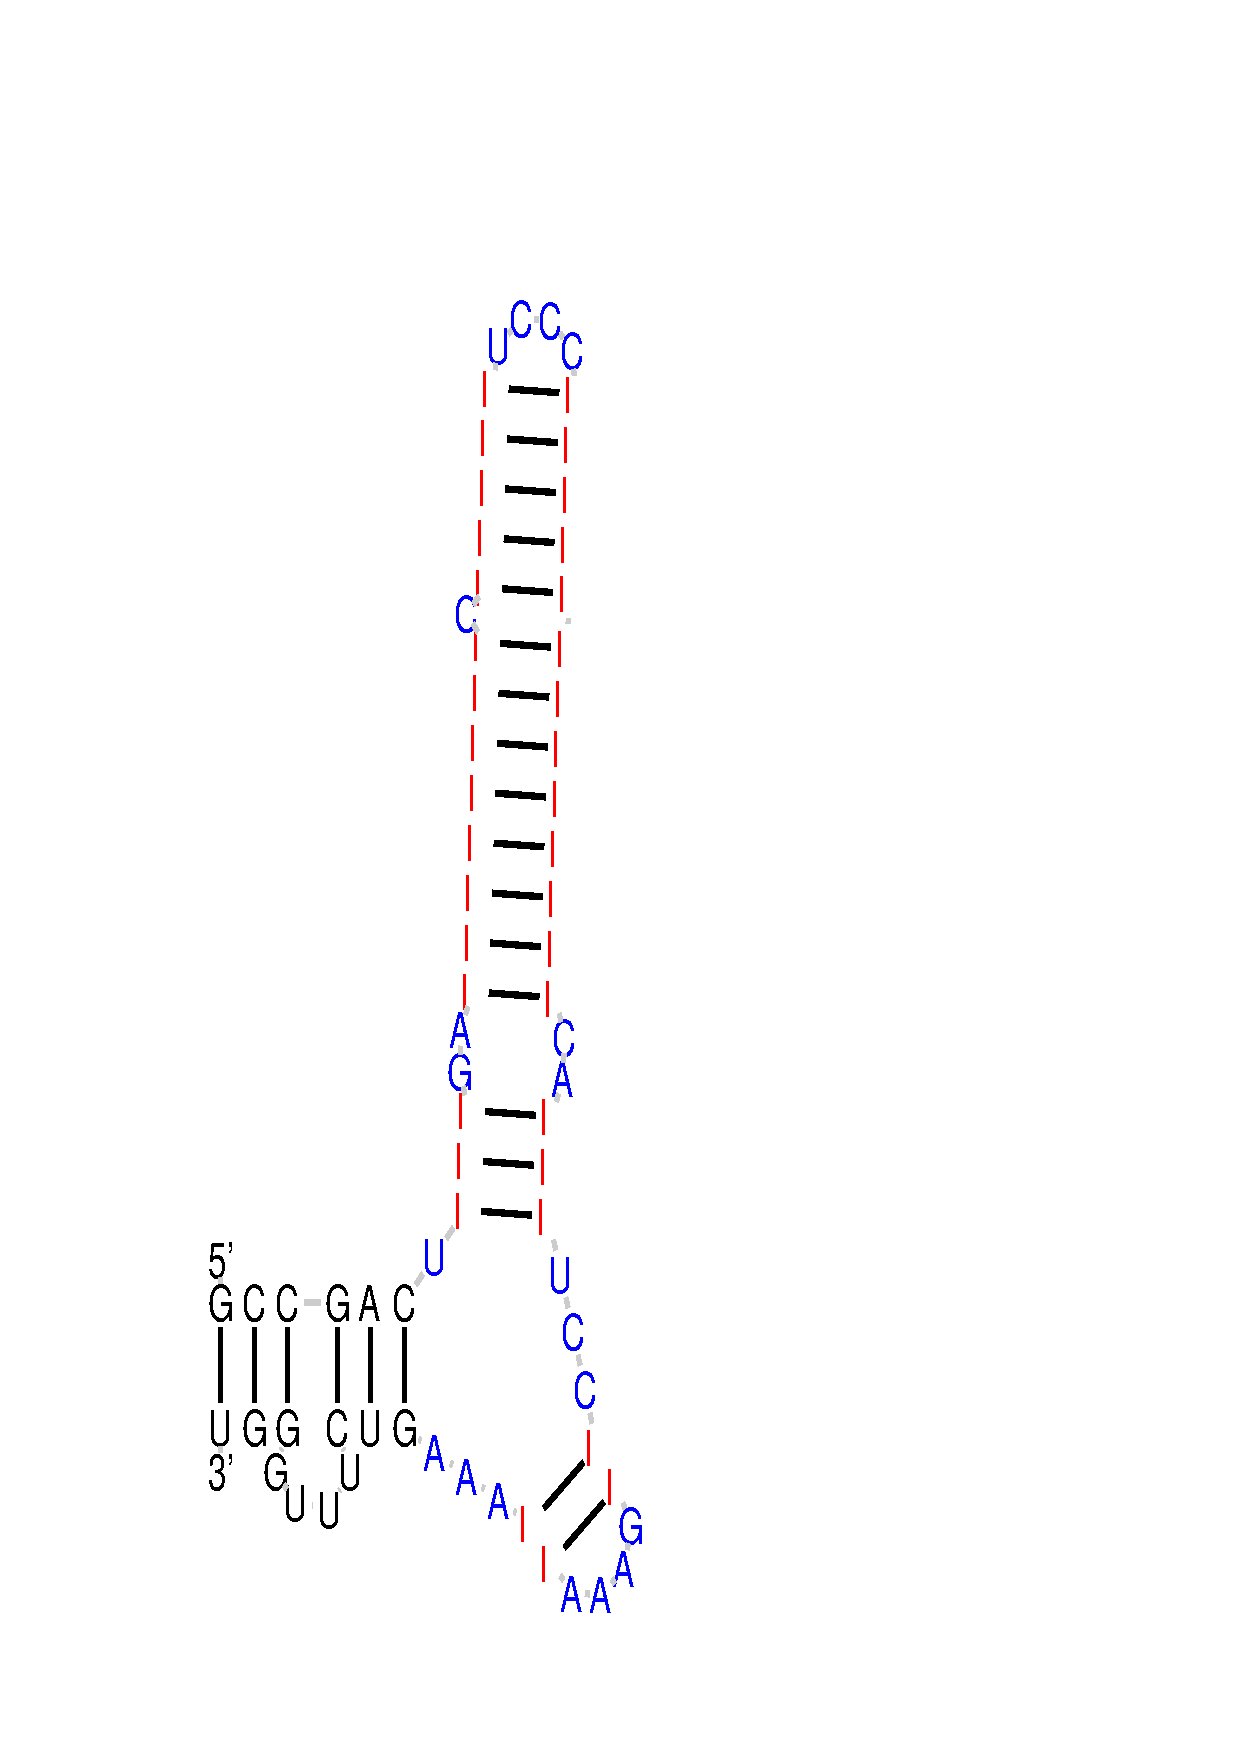
\includegraphics[clip, trim=1cm 21cm 14cm 2.5cm, width=0.85\textwidth]{../img/alg/insert/2/multibranch-del-ins}
    \caption{}
    \label{obr:delete_insert_multibranch_stem_c}
  \end{subfigure}
  \caption{Inverzné operácie: rekonštrukcia stemu}
  \label{obr:delete_insert_multibranch_stem}
\end{figure}

Obrázkom \ref{obr:delete_insert_multibranch_stem} sme simulovali mazanie a~opätovné vkladanie
bázových párov do stemu.
Najprv sme si vytvorili vstupné súbory pre šablónu (obrázok
\ref{obr:delete_insert_multibranch_stem_a} spolu s~fasta súborom)
a cieľovú molekulu (fasta súbor reprezentujúci sekundárnu štruktúru
\ref{obr:delete_insert_multibranch_stem_b}). Následne sme spustili program
s výsledkom na obrázku \ref{obr:delete_insert_multibranch_stem_b}.
Po úspešnej vizualizácií sme skúsili vymeniť šablónovú a cieľovú molekulu
a tým sa pokúsiť znovu vytvoriť pôvodný obrázok. Výsledok môžeme vidieť
na obrázku \ref{obr:delete_insert_multibranch_stem_c}.
Pre lepšie zvýraznenie sme znovu vkladané bázy označili písmenom 'I'.

Tento príklad má za cieľ ukázať, že vieme znovu nakresliť pôvodnú štruktúru
stemu a loopov iba s~malými zmenami v~pozícií
nukleotidov (výsledné loopy sú trochu plytšie ako pôvodné)

Ďalším pokusom bolo znovu vytvorenie celej multibranch loopy.
Na to sme použili rovnakú štruktúru a zmazali z~nej obidva celé
stemy a~nechali sme ju nakresliť naším programom
(obrázok \ref{obr:delete_insert_multibranch_loop_b}).
Následne sme postupovali podobne ako v~prvej simulácií - vymenili
sme šablónovú molekulu s~cieľovou. Výsledkom bol obrázok
\ref{obr:delete_insert_multibranch_loop_c}.

V~tomto príklade je rozdielov vo výslednej vizualizácií oproti pôvodnému nakresleniu
viac, napríklad vrchný stem je oveľa viac vychýlený. Kým v~takejto malej štruktúre
nám to nevadí, pri veľkých už problémy nastávajú, ako ukážeme neskôr.

\begin{figure}[t!H]
  \centering
  \begin{subfigure}[t]{0.3\textwidth}
%trim=left bottom right top
    \includegraphics[clip, trim=1cm 21cm 14cm 2.5cm, width=1\textwidth]{../img/alg/insert/3/multibranch-beg}
    \caption{}
    \label{obr:delete_insert_multibranch_loop_a}
  \end{subfigure}
  \begin{subfigure}[t]{0.3\textwidth}
%trim=left bottom right top
    \includegraphics[clip, trim=0 -2cm 7cm 20cm, width=1\textwidth]{../img/alg/insert/3/multibranch-del}
    \caption{}
    \label{obr:delete_insert_multibranch_loop_b}
  \end{subfigure}
  \begin{subfigure}[t]{0.3\textwidth}
%trim=left bottom right top
    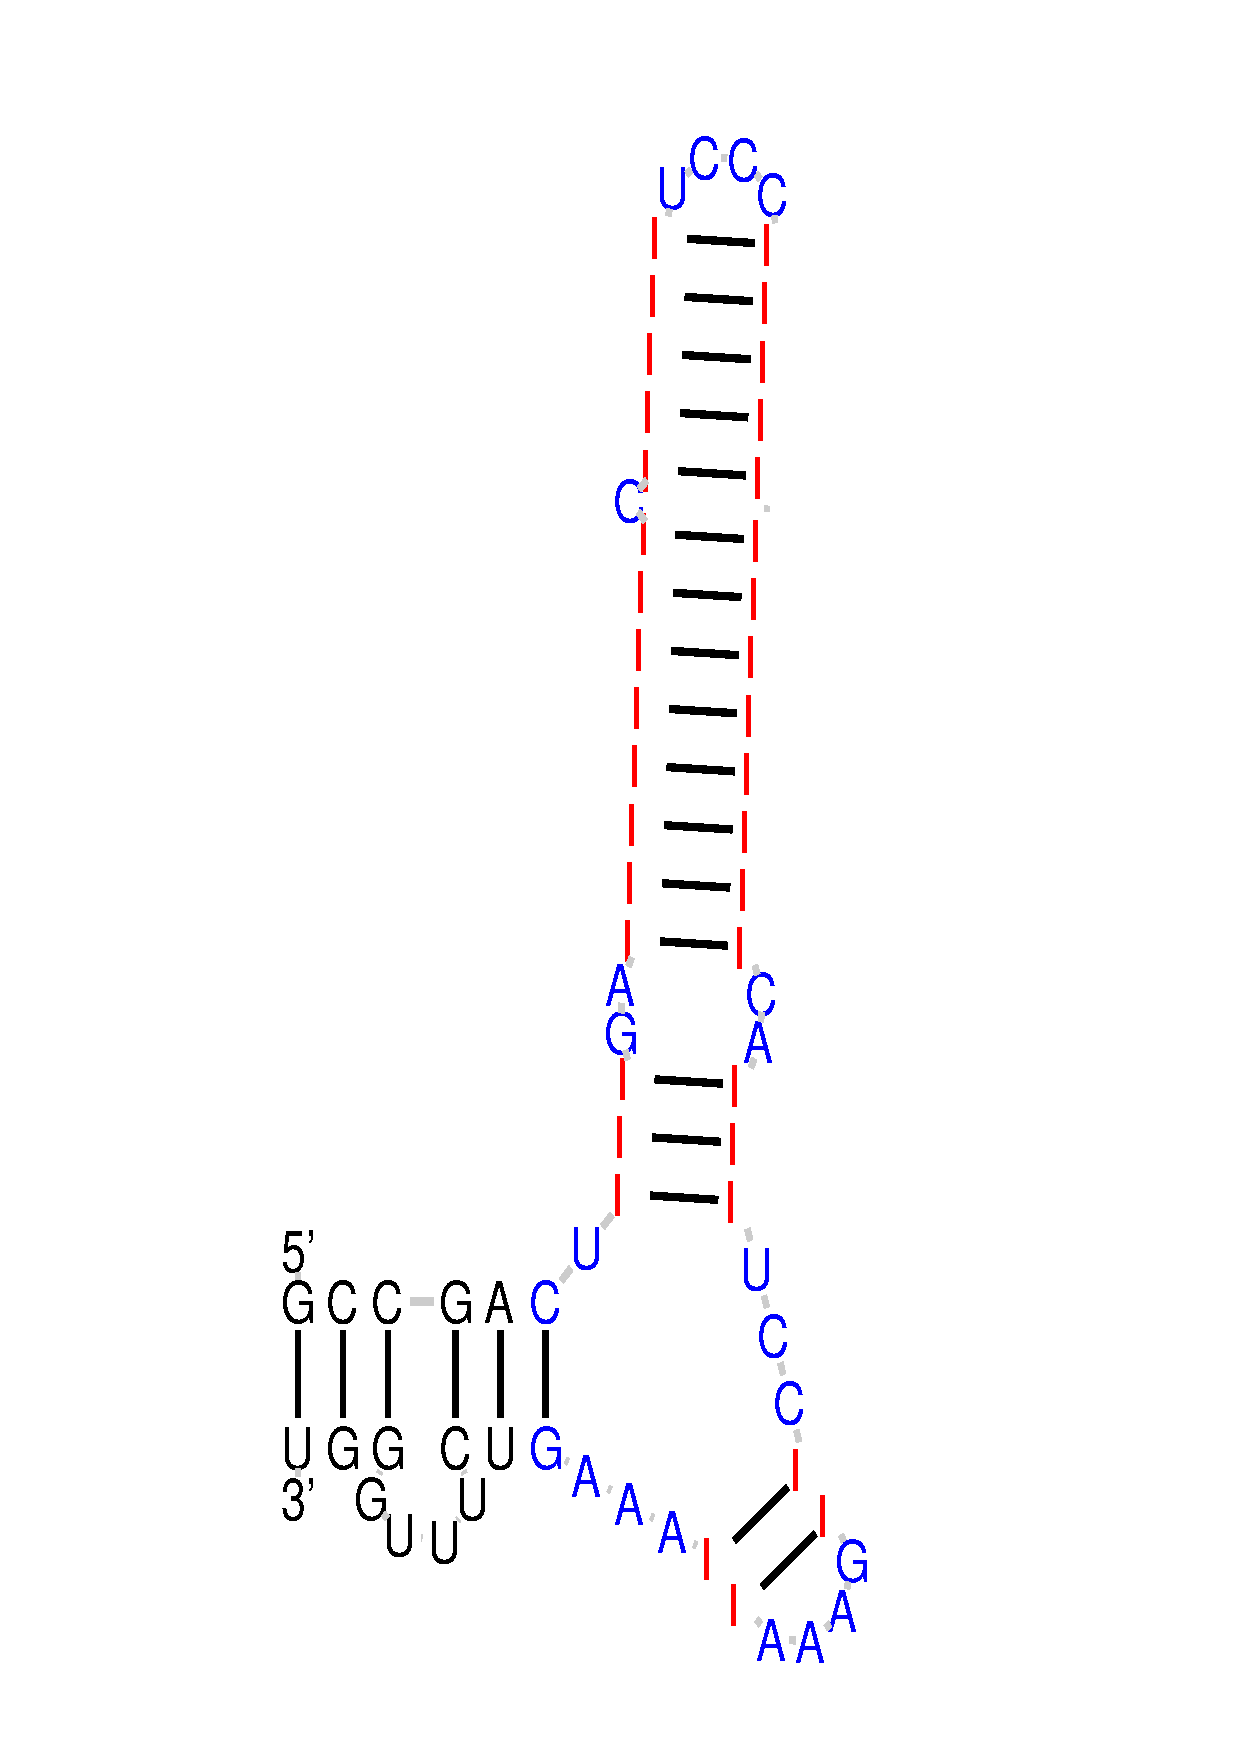
\includegraphics[clip, trim=0 0 0 2cm, width=1\textwidth]{../img/alg/insert/3/multibranch-del-ins}
    \caption{}
    \label{obr:delete_insert_multibranch_loop_c}
  \end{subfigure}
  \caption{Inverzné operácie: rekonštrukcia multibranch loop}
  \label{obr:delete_insert_multibranch_loop}
\end{figure}




\section{Experimenty na reálnych rRNA}

Ďalšiu pozornosť sme upriamili na testovanie existujúcich molekúl.
Ako testovaciu sadu sme zvolili malú podjednotku 16S ribozomálnej RNA
v~živočíšnej ríši.
Z~CRW databázy (\citet{CRW}) sme získali 16 nakreslených molekúl spolu s ich
primárnou a sekundárnou štruktúrou.

Databáza nám ponúka viac formátov sekundárnej štruktúry (BPSEQ, CT, RNAML, BRACKET).
Môžeme sa rozhodnúť, či chceme pracovať s~pseudouzlami, alebo nie.

Zdrojom primárnej štruktúry nám bol RNAML formát, ktorý ju v~sebe ukrýva%
\footnote{Všetky spomenuté formáty okrem dot-bracket obsahujú okrem
sekundárnej štruktúry aj sekvenciu RNA}.
Na reprezentáciu sekundárnej štruktúry sme použili formát dot-bracket.
Počiatočná zvýšená pracnosť súvisiaca s~používaním dvoch typov súborov
sa vyplatila a~výmenou za ňu sme získali pohodlie pri ladení a~testovaní
aplikácie spojené s~ľahkou orientáciou v~štruktúre.

Vizualizačný test sme spustili vo forme každý s každým, teda zo
16 molekúl sme získali 256 nakreslení, u ktorých sme sledovali
hlavne zachovanie ich rovinnosti (výsledná vizualizácia bola bez krížení).

\begin{figure}
  \includegraphics[width=1\textwidth]{../img/statistika/prekryvy-pocetmolekul}
  \caption{Počet prekryvov v testovaných molekulách}
  \label{obr:statistika_prekryvy}
\end{figure}

Graf \ref{obr:statistika_prekryvy} nám popisuje celkové výsledky testu.
Aj keď je veľké množstvo molekúl bez prekryvov, stále je relatívne veľa tých,
u~ktorých sa nám zachovať rovinnosť nakreslenia nepodarilo.
Po použití operácie prekresľovania multibranch loop sme zaznamenali
zvýšený výskyt prekryvov. Závislosť medzi použitím tejto operácie
a~počtom prekryvov nám vyjadrujú ďalšie dva grafy,
prvý - \ref{obr:statistika_prekryvy_s_rotaciami} nám ukazuje, že ak
program musel rotovať a~prekreslovať multibranch loopy,
nedarilo sa mu najlepšie. Naopak, ak berieme do úvahy iba vizualizácie bez
prekresľovania multibranch loopy (graf \ref{obr:statistika_prekryvy_bez_rotacii}),
vidíme, že prekryvy vznikali iba ojedinele.

\begin{figure}
  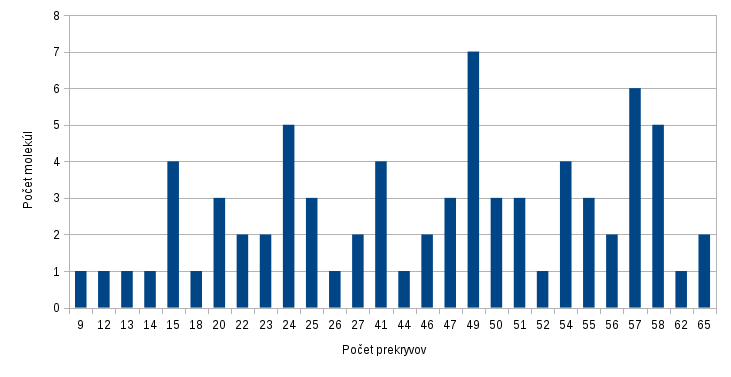
\includegraphics[width=1\textwidth]{../img/statistika/prekryvy-pocetmolekul-s-rotaciami}
  \caption{Počet prekryvov: molekuly, ktoré potrebovali prekreslit multibranch loop}
  \label{obr:statistika_prekryvy_bez_rotacii}
\end{figure}

\begin{figure}
  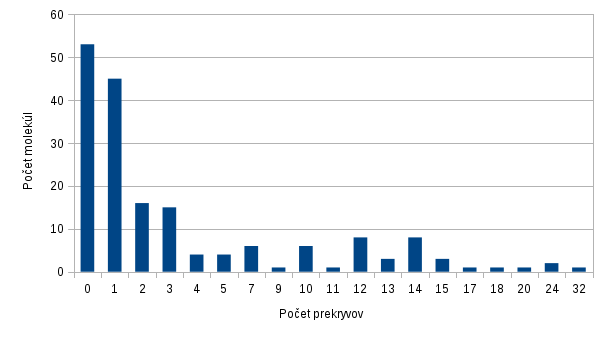
\includegraphics[width=1\textwidth]{../img/statistika/prekryvy-pocetmolekul-bez-rotacii}
  \caption{Počet prekryvov: molekuly bez prekreslovania multibranch loop}
  \label{obr:statistika_prekryvy_s_rotaciami}
\end{figure}

Ďalším faktorom, ktorý ovplyvňuje počet prekryvov je vzdialenosť \textit{tree-edit-distance}.
Od počtu úprav obrázka závisí počet prekryvov, ktoré môžu pri nich vzniknúť.
Túto závislosť nám vyjadruje tabuľka \ref{tab:statistika_prekryvy}.
Pre každú dvojicu molekúl sme si spočítali vzdialenosť medzi nimi.
Poradie je v~závislosti od TED vzdialenosti medzi molekulami%
\footnote{1. je najbližšia (najmenšia hodnota TED), 15. je najvzdialenejšia}

\begin{table}
  \centering
  \begin{tabular}{c|c|c|c}
    \toprule
    \mc{\textbf{Poradie}}  & \mc{\textbf{TED}}          & \mc{\textbf{Počet}}     & \mc{\textbf{Smerodajná}}   \\
    \mc{}                  & \mc{\textbf{(priemer)}}    & \mc{\textbf{prekryvov}} & \mc{\textbf{odchýlka}}     \\
    \midrule
    1   & 85,94   & 5,13  & 1,64  \\
    2   & 113,94  & 13,56 & 11,50 \\
    3   & 137,38  & 12,88 & 8,81  \\
    4   & 158,38  & 11,94 & 7,48  \\
    5   & 172,00  & 13,38 & 9,57  \\
    6   & 189,13  & 15,88 & 13,83 \\
    7   & 196,31  & 14,31 & 11,08 \\
    8   & 199,44  & 13,75 & 10,16 \\
    9   & 258,31  & 14,50 & 13,14 \\
    10  & 262,88  & 14,13 & 12,47 \\
    11  & 265,25  & 14,50 & 13,14 \\
    12  & 271,13  & 15,75 & 13,60 \\
    13  & 301,19  & 25,25 & 0,66  \\
    14  & 345,25  & 30,38 & 1,81  \\
    15  & 805,63  & 15,25 & 0,66  \\
    \bottomrule
  \end{tabular}
  \caption{Počty prekryvov v~závislosti od tree-edit-distance vzdialenosti}
  \label{tab:statistika_prekryvy}
\end{table}

Zaujímavosťou je, že ku všetkým molekulám bola najvzdialenejšia (pätnásta v~poradí)
molekula \textit{Echinococcus granulosus (U27015)} s~priemernou TED
vzdialenosťou $805,63$ a~odchýlkou $12,92$.





\section{Chyby}

V~tejto kapitole uvedieme vygenerované obrázky niektorých molekúl a~na nich ukážeme časté problémy,
ktoré pri vizualizácii nastavali.

\subsection{Otáčanie vetvy kvôli existujúcej hrane}

Jedným príkladom za všetky je molekula rRNA medúzy (\textit{L10829},
obrázok \ref{obr:chyba_otocenie_vetvy_povodna})
Po tom, čo sme skúsili nakresliť molekulu samu na seba
(vzorová aj cieľová molekula bola medúza) vznikol problém,
kedy sa celá jedna vetva molekuly otočila na jednu stranu.
Je to spôsobené existenciou bázového páru,
ktorý je v~pôvodnej molekule znázornený dlhšou lomenou čiarou
a~keďže náš program normalizuje všetky vzdialeností medzi bázovými
pármi s~následným vyrovnávaním stemov, vznikajú aj obrázky
podobné \ref{obr:chyba_otocenie_vetvy}.

\begin{figure}
  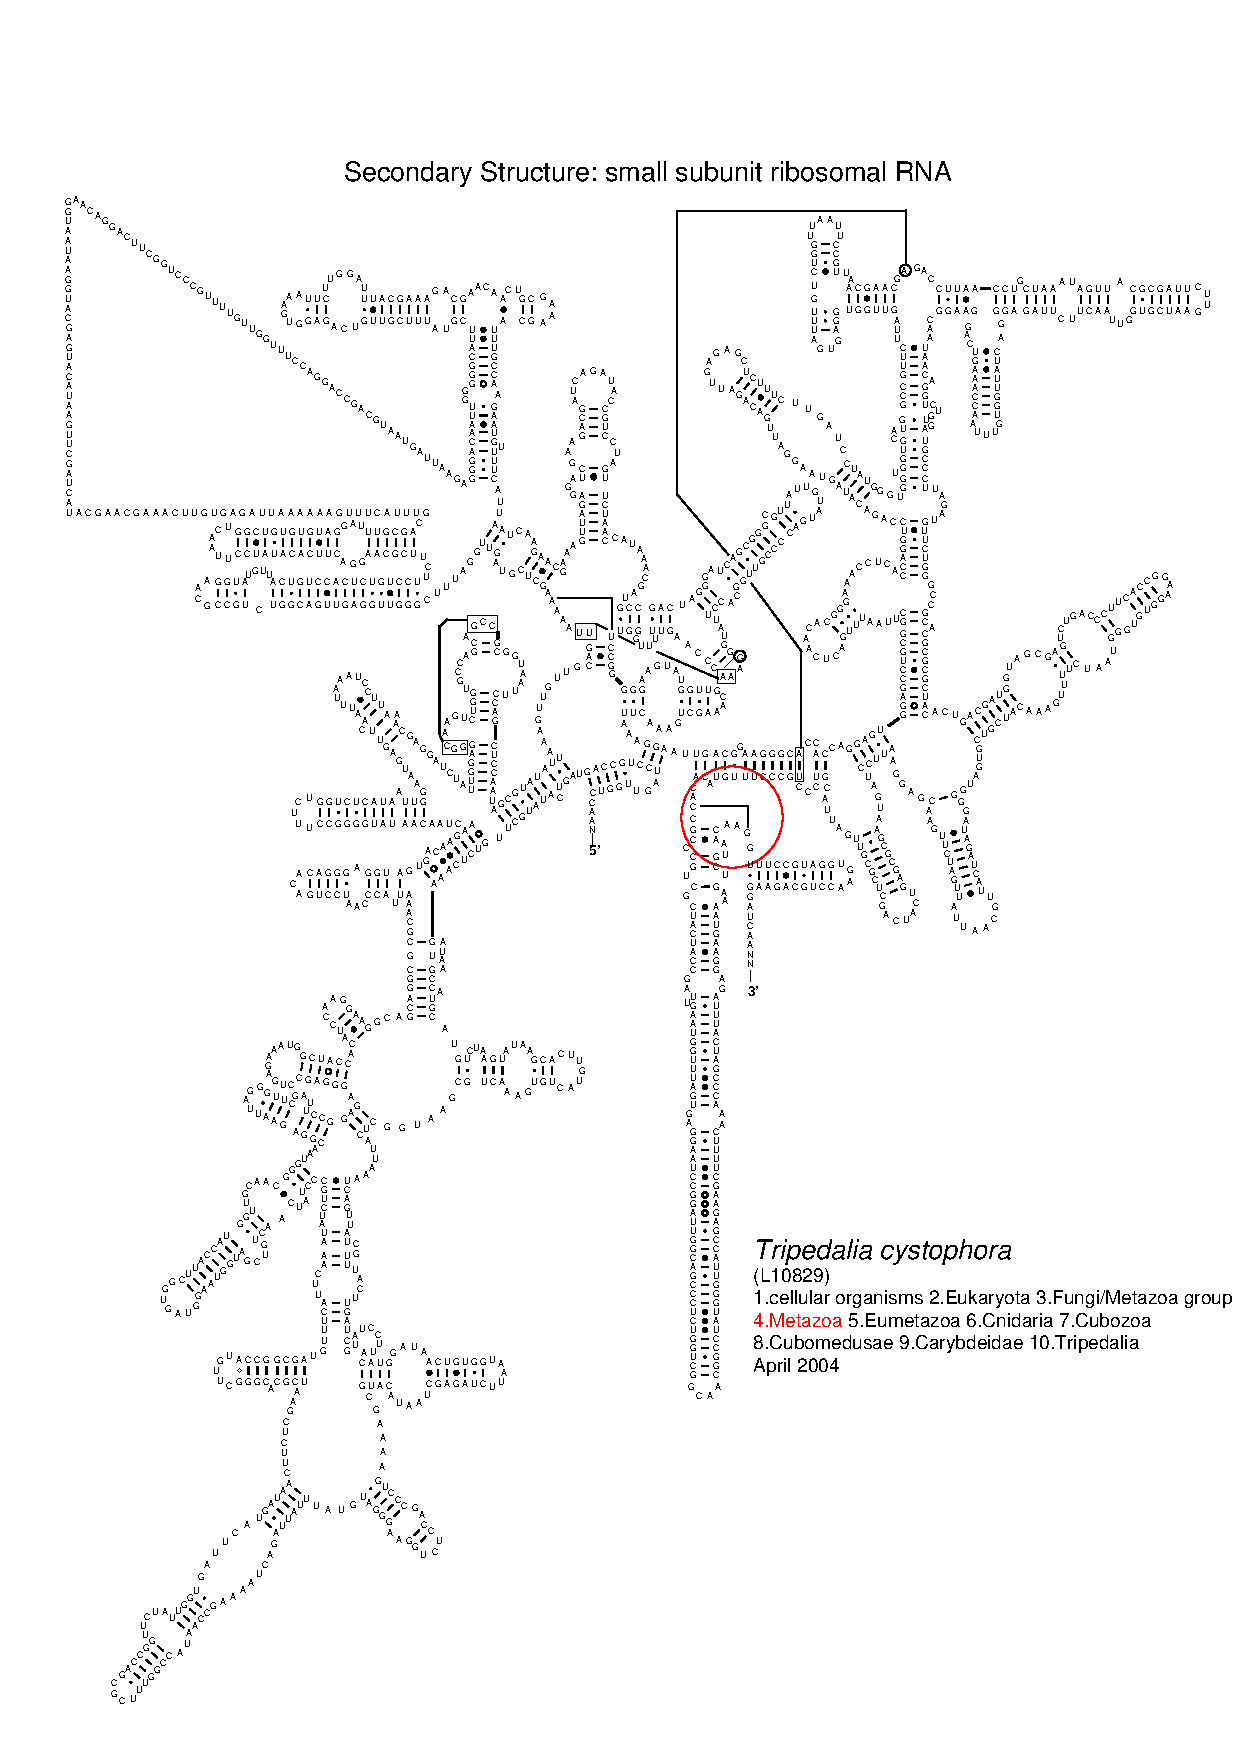
\includegraphics[width=1\textwidth]{../img/chyby/tripedalia_cystophora}
  \caption{Pôvodná vizualizácia rRNA medúzy (\textit{L10829})}
  \label{obr:chyba_otocenie_vetvy_povodna}
\end{figure}

\begin{figure}
%trim=left bottom right top
  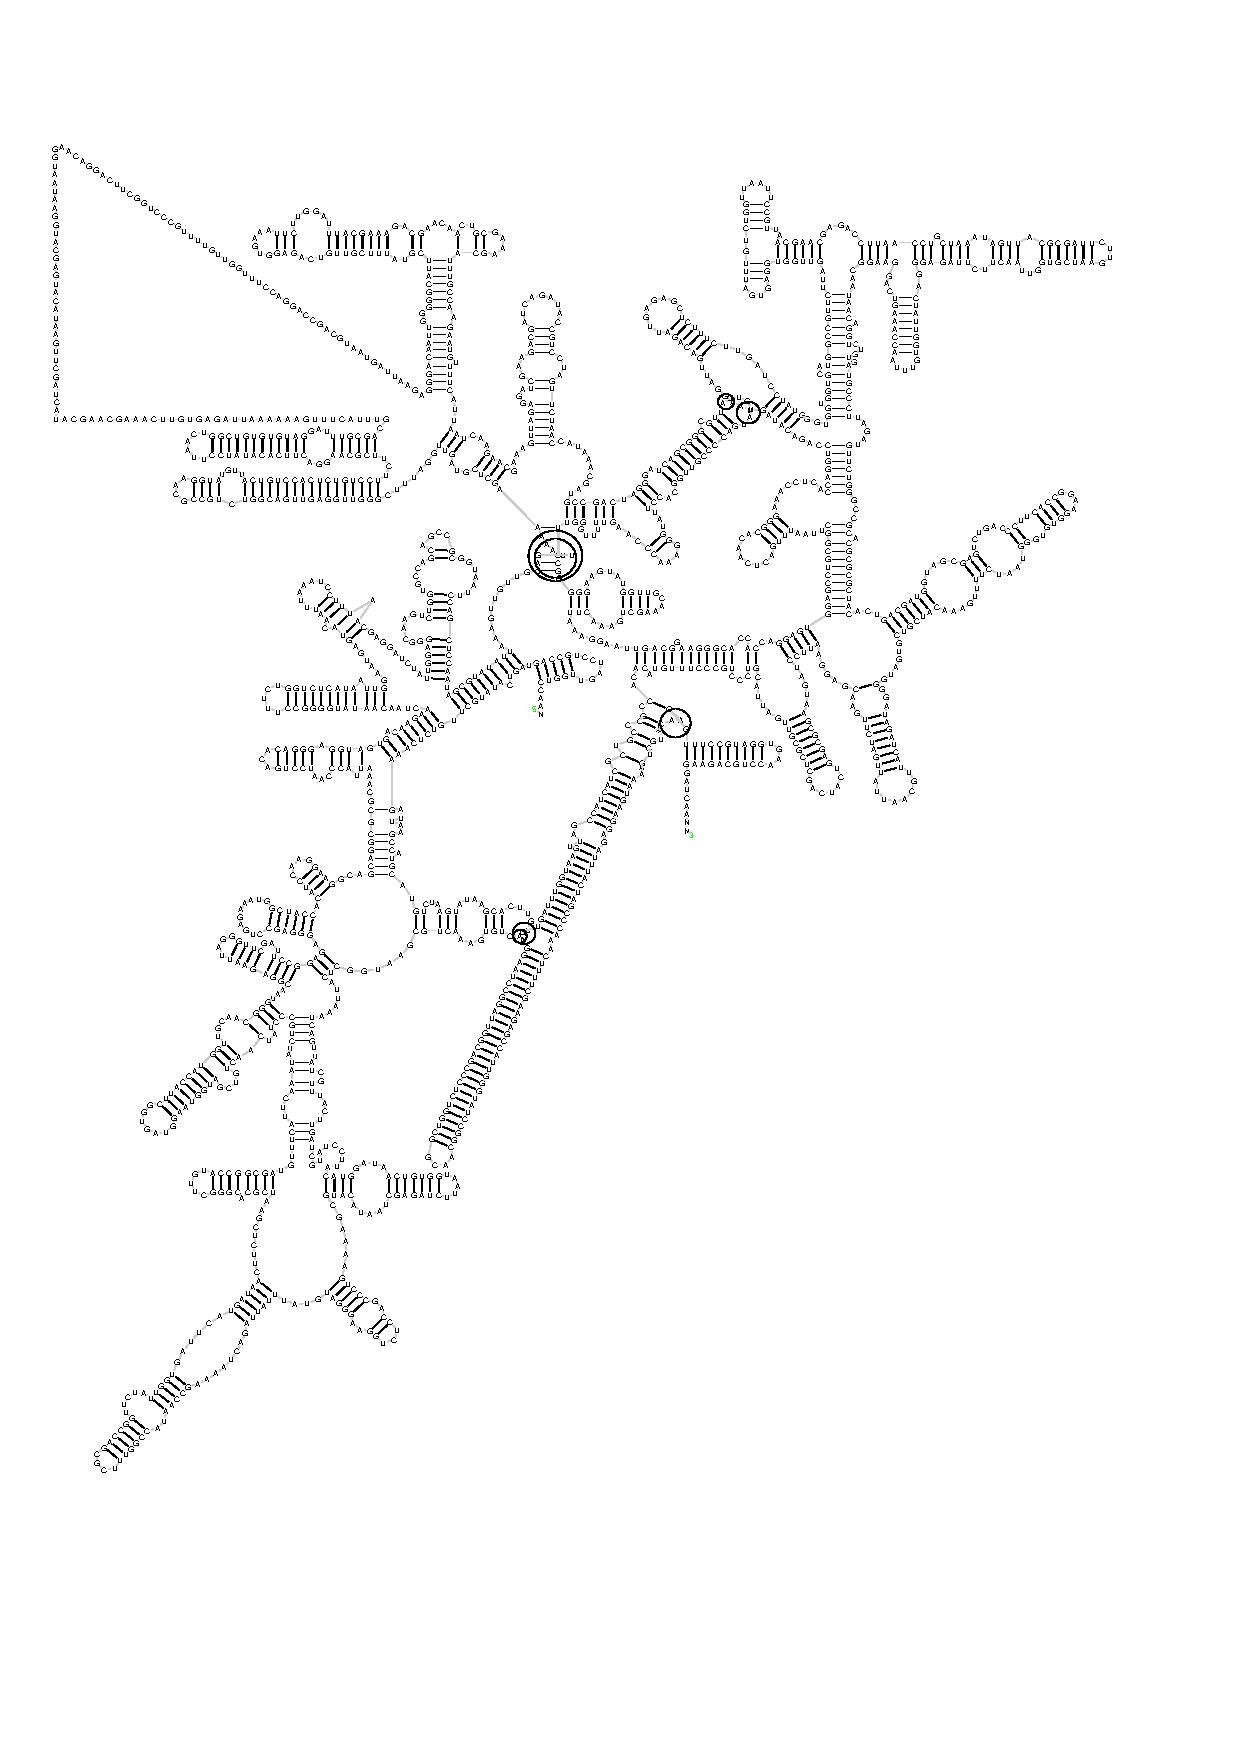
\includegraphics[clip, trim=0 4cm 2cm 2cm, width=1\textwidth]{../img/chyby/tripedalia_cystophora-tripedalia_cystophora}
  \caption{Vizualizácia rRNA medúzy pomocou seba samej ako vzoru}
  \label{obr:chyba_otocenie_vetvy}
\end{figure}

\subsection{Rozloženie báz na kružnicu}

Niekedy sa prekresleniu celej loop nevyhneme, ak napríklad vkladáme veľmi veľké množstvo nukleotidov na jedno
miesto. Vtedy dochádza k~problémom načrtnutým na obrázku \ref{obr:chyba_rozloženie_loopy}.
Na tomto konkretnom príklade je nakreslený stem, vo vnútri ktorého je veľka interior loop. Kvôli tomu,
že chceme dodržiavať pravidlá o kružnicovom tvare loopy, nájdeme dostatočne veľkú kružnicu.
V~tomto prípade až príliž veľkú%
\footnote{Vo vrchnej vetve ja taktiež znázornená kružnica, ale oproti spodnej obsahuje iba 2 vrcholy}

\begin{figure}
%trim=left bottom right top
  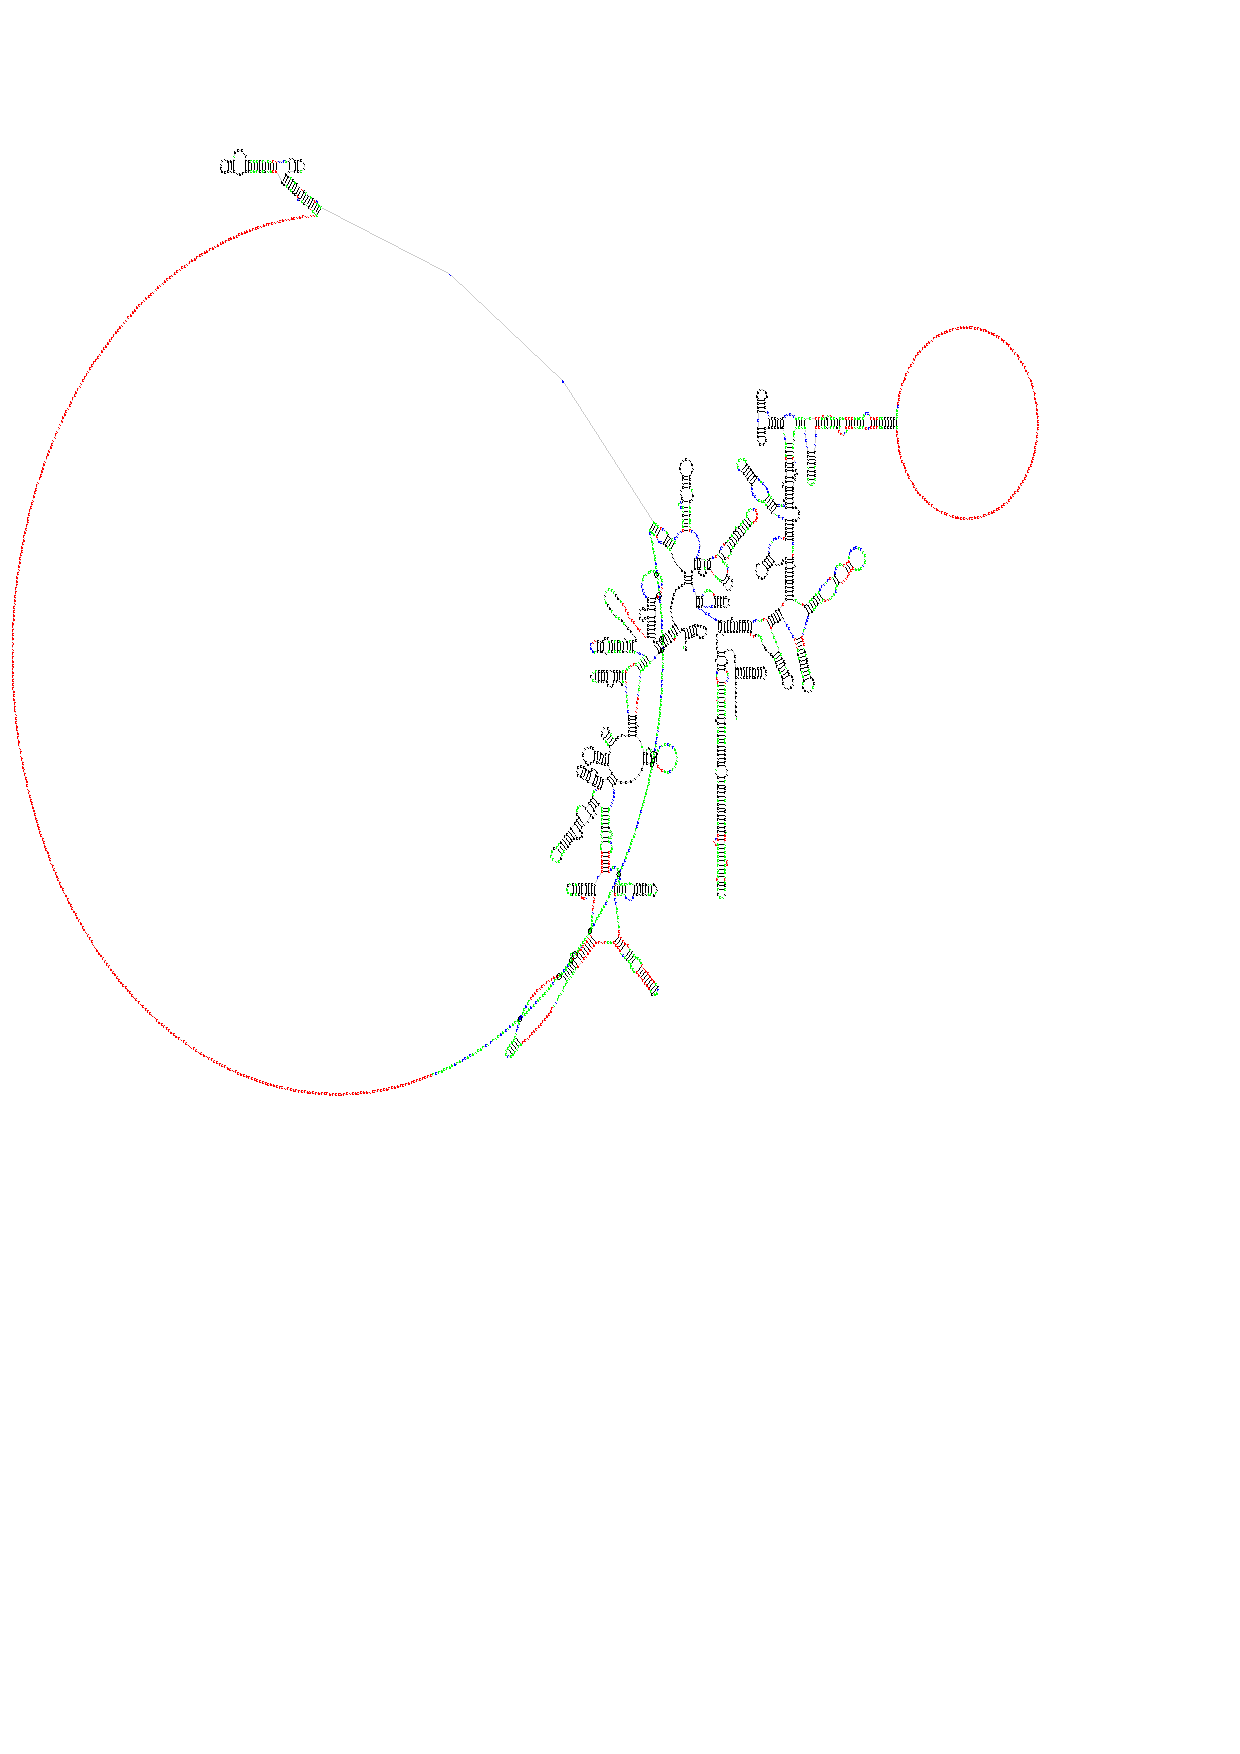
\includegraphics[clip, trim=0 10cm 3cm 2cm,width=1\textwidth]{../img/chyby/african_frog-echinococcus_granulosus}
  \caption{Chyba pri rozkladaní báz na kružnicu}
  \label{obr:chyba_rozloženie_loopy}
\end{figure}

\subsection{Otáčanie vetvy kvôli prekreslovaniu multibranch loopy}

Ako už aj graf na obrázku \ref{obr:statistika_prekryvy_bez_rotacii} ukázal,
prekresľovanie multibranch loopy a~rotácie všetkych vetiev spôsobuje masívne prekryvy.
Podobne ako na obrázku \ref{obr:insert_multibranch}, prekreslenie multibranch loopy
pri vizualizácií RNA mušle (\textit{X53899}) pomocou obrázka RNA cikády (\textit{U06478}).
Na výslednom obrázku \ref{obr:chyba_rotacia_multibranch} sme zvýraznili miesto
uskutočnenej rotácie. Ako vidíme, väčšina prekryvov je spôsobená práve ňou.

\begin{figure}
%trim=left bottom right top
  \centering
  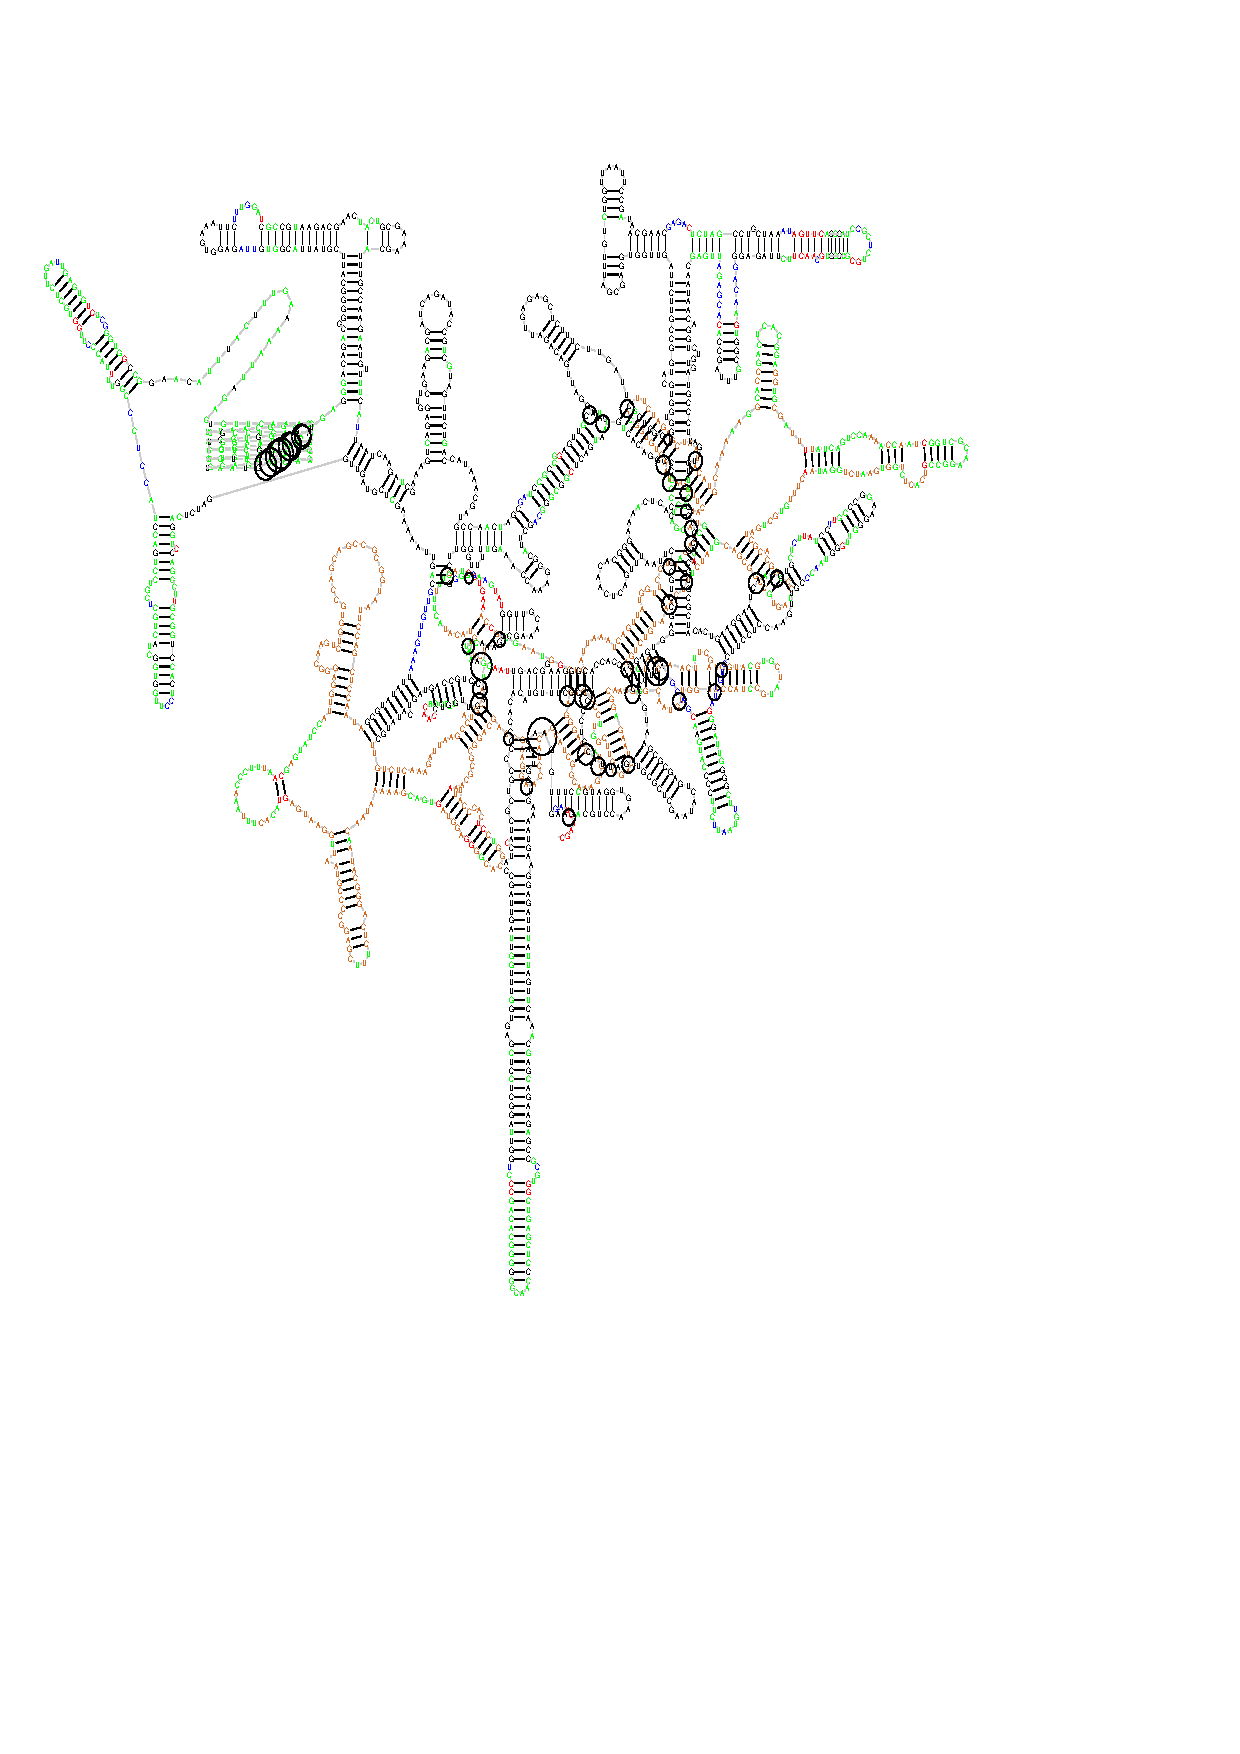
\includegraphics[clip, trim=0.5cm 7cm 4cm 2cm,width=1\textwidth]{../img/chyby/cicadas-sea_scallop}
  \caption{Chyba pri otáčani kvôli prekreslovaniu multibranch loopy}
  \label{obr:chyba_rotacia_multibranch}
\end{figure}









